\section{Reiteration: OU tangle diagrams}

Now we recall a few important concepts from the article \citep{barnatan2020tangles}, on which we base our approach. We define an operation on tangle diagrams, an algorithm, and mention that for the set of diagrams we consider the algorithm does not produce a final result. Instead the algorithm approaches Wild tangles, later we will attempt to describe these wild tangles.

\subsection{The Glide move}

The Glide move as defined in \citep{barnatan2020tangles} is simply an alias for the composition of an R2 and R3 move. We illustrate the Glide move in \Cref{fig:GR2R3}.

\begin{figure}[h!]
\centering
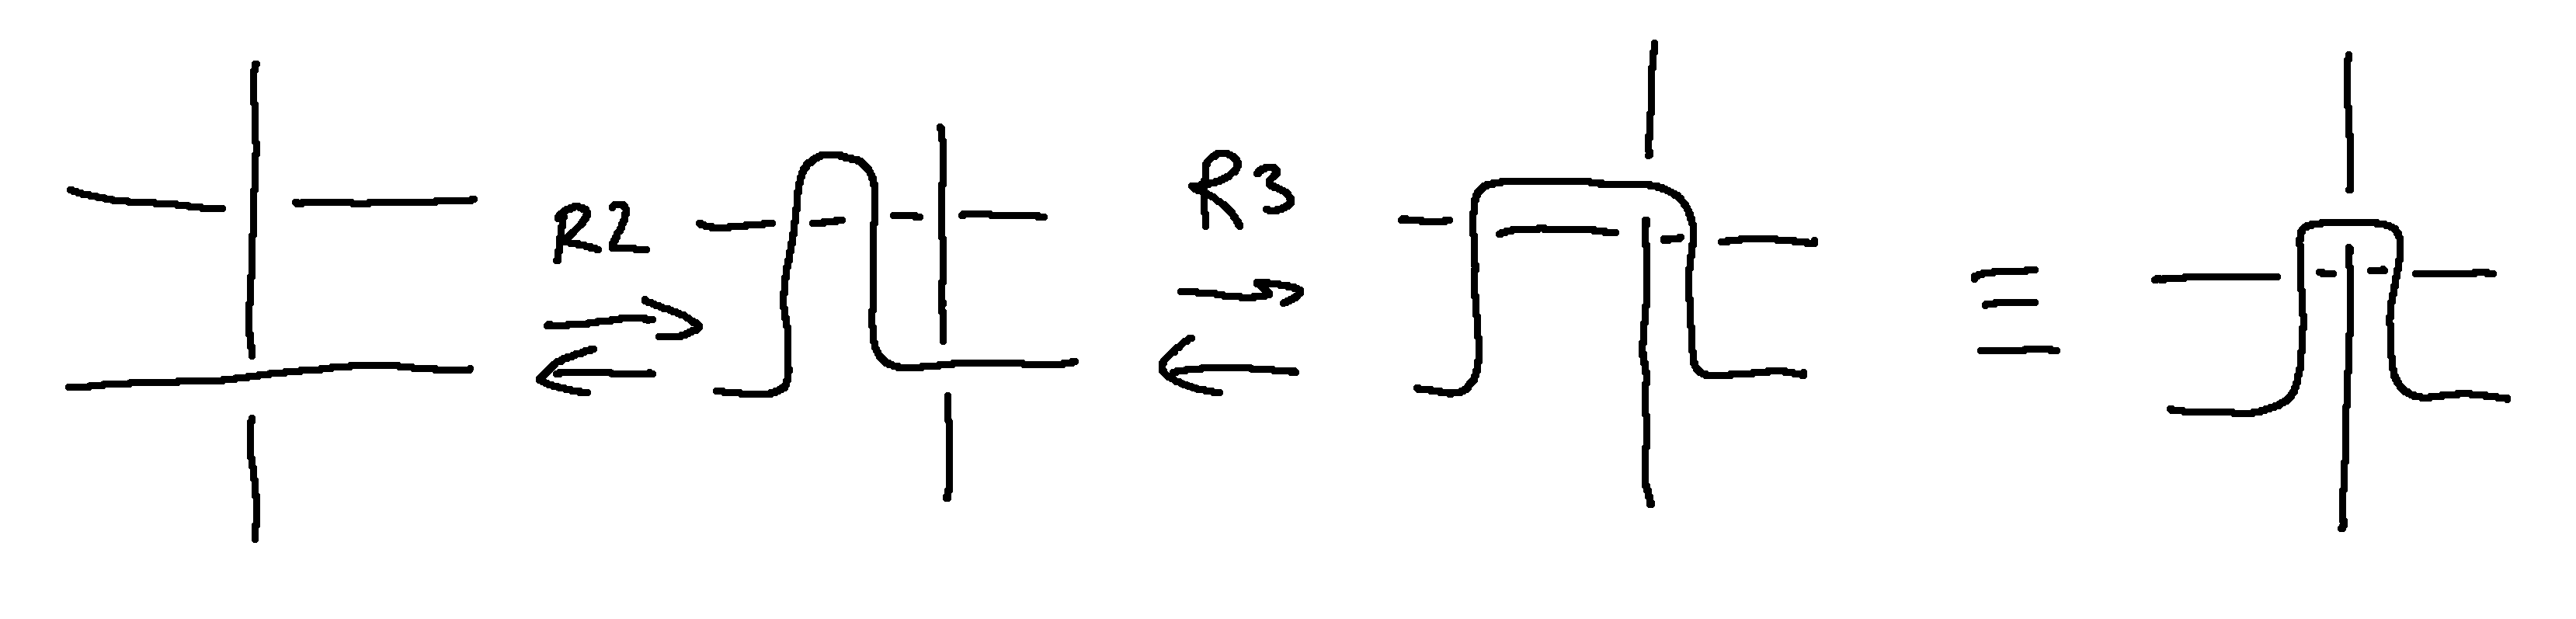
\includegraphics[width=\textwidth]{G=R2+R3.png}
\caption{The Glide move is equivalent to an application of R2 and R3.}
\label{fig:GR2R3}
\end{figure}

The goal of the Glide move is to swap positions of over strands and under strands, i.e. if the Gauss code of a tangle diagram contains $U^s_iO^t_j$ then by a glide move we can swap those symbols to produce a Gauss code with $O^t_iU^s_j$. However this is not the only change the Glide move introduces, other parts of the code are changed since we introduce two new crossings. We can translate the Glide move into an operation on the Oriented Gauss code. This makes it humanly possible to follow the evolution of the diagram upon Gliding. For a tangle diagram with crossings $a,b$ we distinguish 4 cases:
\begin{align*}
U_a^+O_b^-,O_a^+,U_b^-\mapsto O_a^-U_b^+,O_{c}^-O_b^+O_{d}^-,U_{c}^-U_a^-U_{d}^+\\[0.25cm]
U_a^+O_b^+,O_a^+,U_b^+ \mapsto O_a^+U_b^+,O_{c}^+O_b^+O_{d}^+,U_{d}^-U_a^+U_{c}^+\\[0.25cm]
U_a^-O_b^-,O_a^-,U_b^-\mapsto O_a^-U_b^-,O_{d}^+O_b^-O_{c}^+,U_{c}^+U_a^-U_{d}^+\\[0.25cm]
U_a^-O_b^+,O_a^-,U_b^+ \mapsto O_a^+U_b^-,O_{d}^+O_b^-O_{c}^-,U_{d}^+U_a^+U_{c}^-,
\end{align*}
i.e. we replace the substrings of the current Gauss code on the left with their corresponding substrings on the right. We have that $a,b,c,d\in\mathbb N$, the indices $c,d$ can be any number not yet used in the Gauss code. Each case corresponds to a combination of crossing signs, we illustrate the first case in \Cref{fig:glide}.
\begin{figure}[h!]
\centering
\begin{subfigure}{0.40\textwidth}
\centering
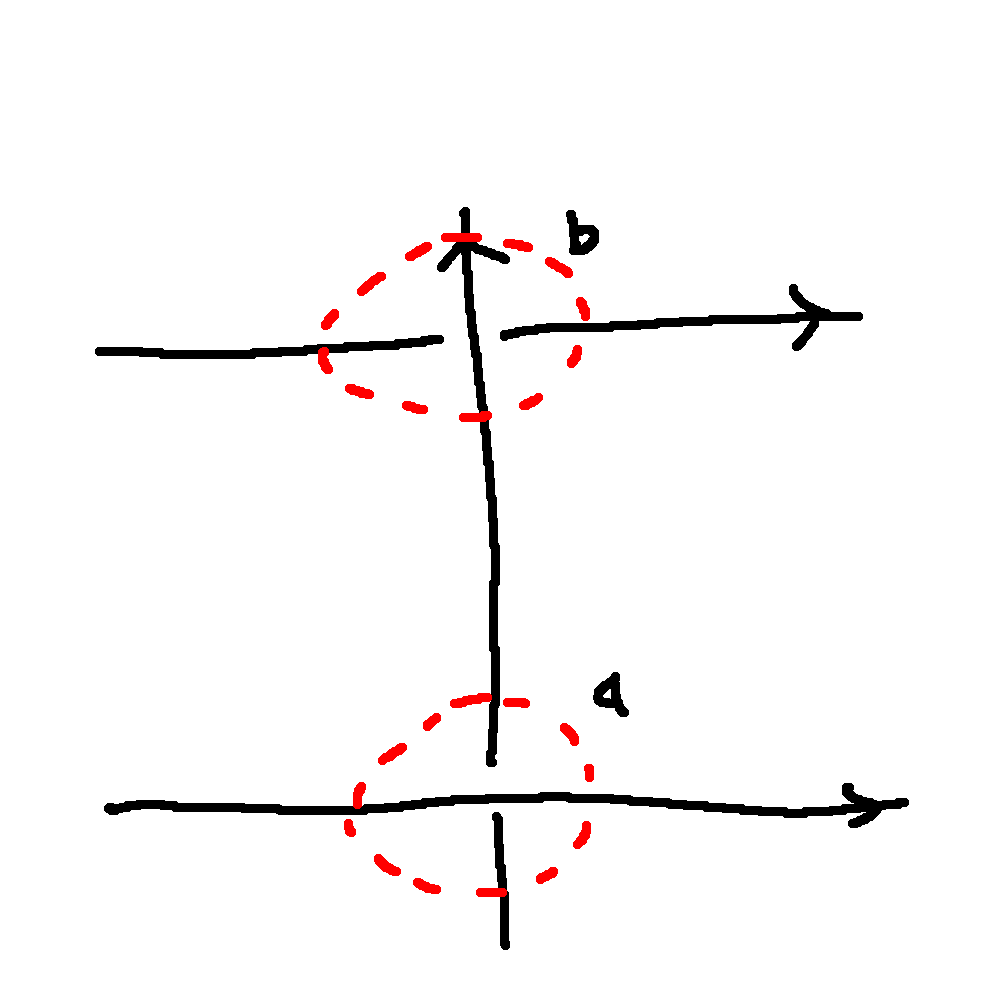
\includegraphics[width=\textwidth]{glide1.png}
\caption{Before applying the Glide move}
\label{fig:glide1}
\end{subfigure}
\hspace{1cm}
\begin{subfigure}{0.40\textwidth}
\centering
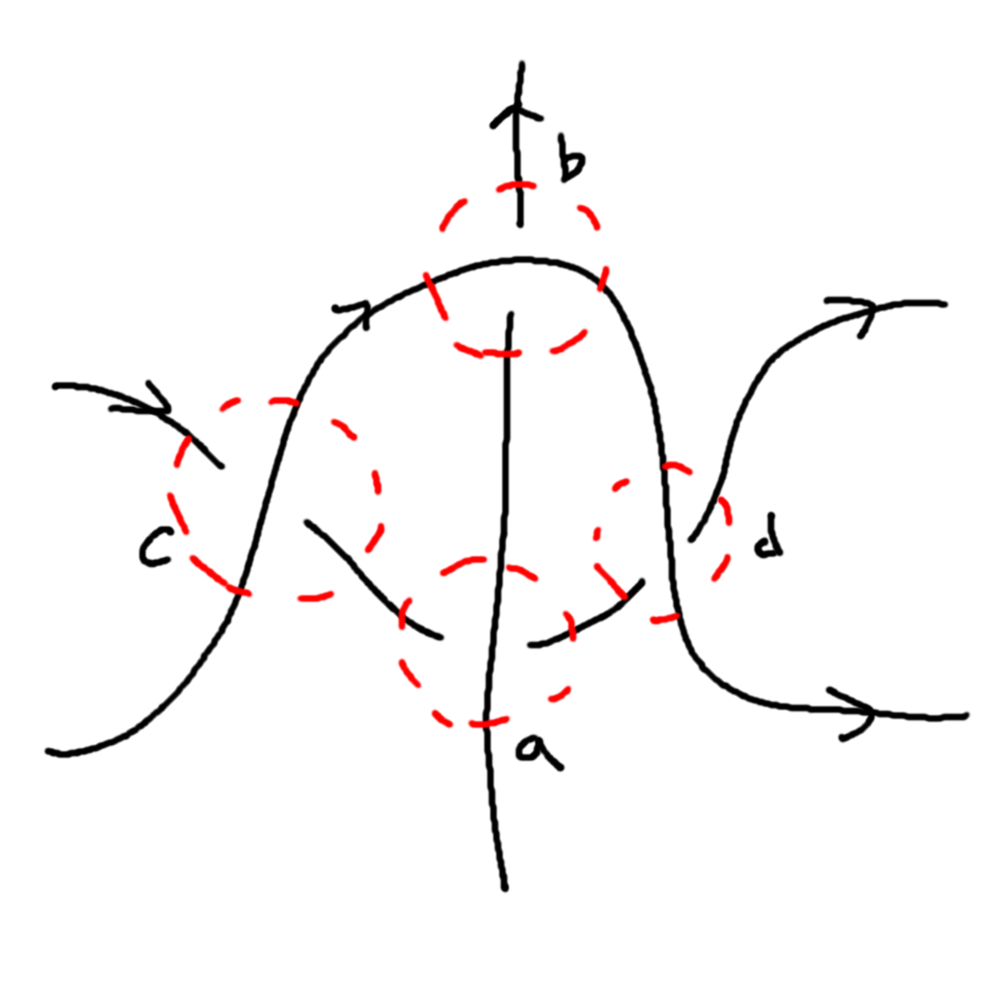
\includegraphics[width=\textwidth]{glide2.png}
\caption{After applying the Glide move}
\label{fig:glide2}
\end{subfigure}
\caption{Example of the Glide move, the triple $U_a^+O_b^-,O_a^+,U_b^-$ are each replaced with $O_a^-U_b^+,O_{c}^-O_b^+O_{d}^-,U_{c}^-U_a^-U_{d}^+$}
\label{fig:glide}
\end{figure}

\subsection{OU Algorithm}
We are now in the position to describe the algorithm from the paper:
\begin{enumerate}
\item For each string in order of occurrence in the Gauss code of the tangle, check each pair of consecutive symbols 
\item If we encounter a pair $U^s_iO^t_j$, apply the Glide move,
\item Simplify the diagram by R1 and R2 moves,
\item If the diagram is in an OU form, we are done, if not return to step 1.
\end{enumerate}

We will proceed in the same way except we will skip step 3. We are more interested in the patterns that arise from iterations of the Glide move, step 3 removes R1 and R2 ``artifacts" in a mostly arbitrary way, in a way we cannot easily follow. Not reducing by R1 and R2 moves should make it simpler to conjecture statements.

For a tangle diagram $D$ we write $\Gamma(D)$ to represent the diagram resulting from the application of the OU Algorithm on $D$. We would hope to see that for each diagram $D$ there exists a $\Gamma(D)$, however it is shown in Theorem 2.3 of \citep{barnatan2020tangles}  that $\Gamma(D)$ only exists for diagrams that are \textit{acyclic}.  

\subsection{Acyclic Diagrams}

\begin{definition}\textbf{(Cyclic Tangle Diagrams)}
A ``cascade path" is a path on the tangle diagram that begins on one of the strands, follows the orientation of the strand it is on, and at a crossing may drop from the upper strand to the lower strand, if desired. A \textit{closed} cascade path is one that returns to its starting position. A diagram is \textit{cyclic} if there exists a closed cascade path, a diagram that is not cyclic is called \textit{acyclic}. 
\end{definition}

An example of an acyclic diagram is given in \Cref{fig:exampletangle} and a cyclic diagram in \Cref{fig:trefexample}. The diagram in \Cref{fig:exampletangle} contains paths that return to the same crossing, however none of them are cyclic since to close the path it is required to jump from an under strand to an over strand. Conversely, on \Cref{fig:trefexample} we have a cycle by:
\begin{enumerate}
\item start on the over strand of crossing 3,
\item follow the orientation through crossing 1,
\item at crossing 2 we are on the over strand, and we choose to jump to the under strand,
\item following the under strand of 2, we arrive at the over strand of 3, where we started.
\end{enumerate}

So we have a criteria for when the OU algorithm terminates for a given tangle diagram. For the case of 1-tangle diagrams we can deduce some information about OU forms before invoking the acyclic property.

\begin{theorem}
All OU tangle diagrams of 1 strand are equivalent by Reidermeister moves to the trivial tangle diagram.
\end{theorem}

\begin{proof}
Consider an OU tangle diagram of 1 strand. Since it is OU, we can split the strand into two parts, one which consists of all over strands, and one with all under strands. Having split the strand into two parts, we notice that the parts are independent of one another, i.e. since the pieces are either all over or all under, they have no interconnections or flips due to crossings. Finally, we can reshape each piece independently to form a straight line, and in the process remove all the crossings. Hence we have a trivial tangle.
\end{proof}

\subsection{Retrospect and further considerations}

So if we encounter an OU 1-tangle diagram, there is nothing much to discuss, the distinction is not useful, since trivial tangle diagrams form only a small proportion of all tangle diagrams. The converse of the statement is not true however, a trivial tangle diagram can also be non OU, simply consider the tangle containing a single Reidermeister 1 move (refer to \Cref{fig:R1move} the bottom  diagram with UO), and here the cyclic property helps distinguish these cases. 

We had made the decision to not reduce by R1 and R2 moves, however this produces issues with the original implementation of the Glide move, specifically, there is a family of tangle diagrams for which the Glide move is not well defined. For example in \Cref{fig:pathology} the OU algorithm will not successfully make a glide move, since the move tries to swap the crossing with itself. As we push the crossing along the under strand, the over strand retreats equally, in such a way we simply circle around indefinitely. Any diagram that contains an R1 move like this will have issues under the OU algorithm, so we decide to ignore crossings like this in step 2 of the algorithm This then implies that in some cases the algorithm can terminate erroneously, which is not a serious problem, since we can simply remove the R1 loop with no issues afterwards.

\begin{figure}
\centering
\begin{subfigure}{0.49\textwidth}
\centering
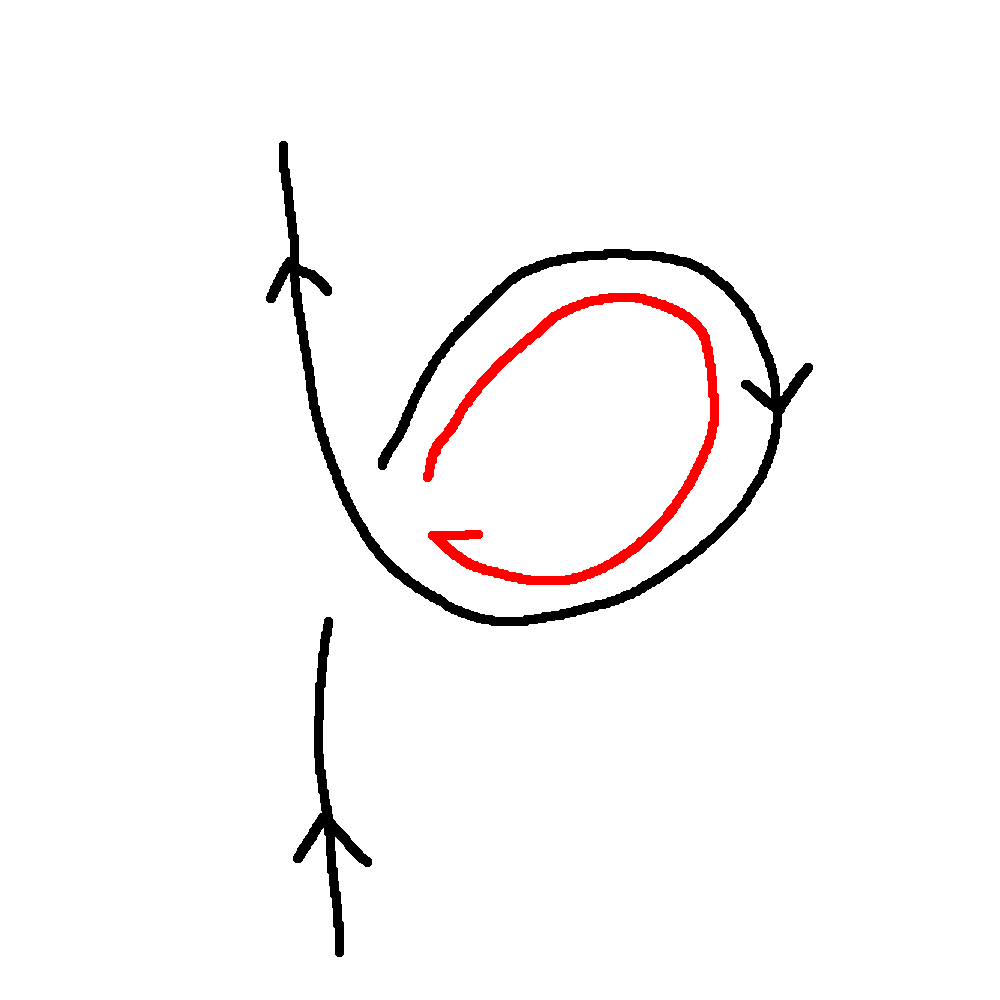
\includegraphics[width=0.7\textwidth]{path1.png}
\end{subfigure}
\hfill
\begin{subfigure}{0.49\textwidth}
\centering
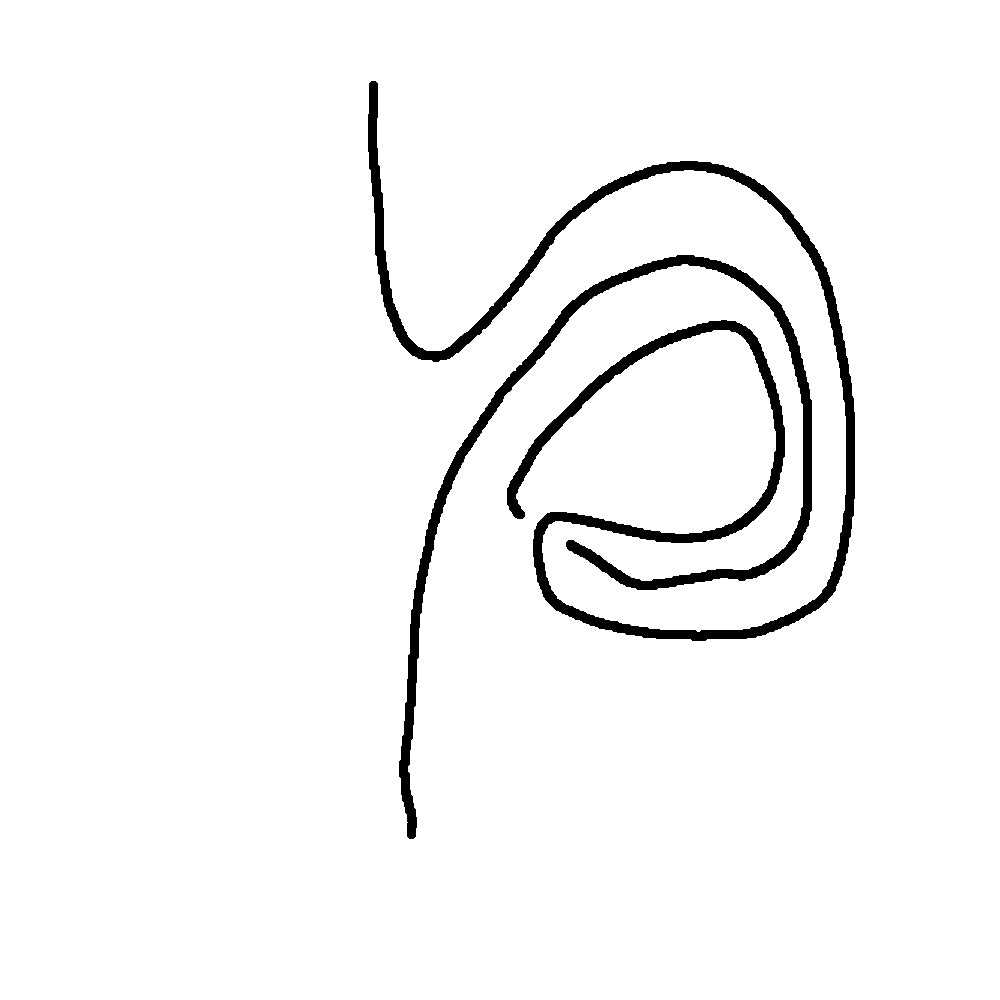
\includegraphics[width=0.7\textwidth]{path2.png}
\end{subfigure}
\caption{A very troublesome tangle}
\label{fig:pathology}
\end{figure}